\documentclass[a4paper]{article}
\usepackage[utf8]{inputenc}
\usepackage[russian]{babel}
\usepackage[warn]{mathtext}

\usepackage{graphicx}
\usepackage{wrapfig}
\usepackage{amsmath}
\usepackage{floatflt}
\usepackage{float}
\usepackage{amssymb}
\usepackage{mathrsfs}

\usepackage{longtable}
\usepackage{multicol}
\usepackage{multirow}

\usepackage{lscape}
\usepackage{hvfloat}

\usepackage{indentfirst}

\usepackage[left=15mm, top=20mm, right=15mm, bottom=20mm, footskip=10mm]{geometry}
\linespread{1.3}
\usepackage{multicol}

\begin{document}
\begin{titlepage}
\noindent

	\centering
	\vspace{2cm}
	{\scshape\LARGE Московский физико-технический институт (НИУ)\par}
	\vspace{1cm}
	{\scshape\Large Лабораторная работа\par}
	\vspace{1cm}
	{\huge\bfseries Атомно-силовой микроскоп\par}
	\vspace{1cm}
	
	\begin{figure}[H]
	\centering
	
\includegraphics[width=0.4\linewidth]{dpqe.jpg}
   	\label{fig:0}
	\end{figure}
	%\vspace{0.5cm}
	\vfill
	
\begin{flushright}
	{\large выполнил студент III-ого курса ФФКЭ, группа 852}\par
	\vspace{0.3cm}
	{\LARGE Андреев Георгий} \par
	\vspace{0.3cm}
	{\large преподаватель}\par
	\vspace{0.3cm}
	{\LARGE Чуприк Анастасия Александровна} \par
\end{flushright}

\vfill

% Bottom of the page
	Долгопрудный, 2020 г.
\end{titlepage}
\newpage
\tableofcontents
\newpage
\section{Цель работы}
\begin{itemize}
	\item Данная лабораторная работа направлена на практическое ознакомление студентов с физическими принципами функционирования атомно-силового микроскопа;
	\item Ознакомление с основными методиками измерения.
\end{itemize}


\section{Теоретическая справка}
\subsection{Основная концепция работы АСМ}

Физика поверхностных явлений в настоящее время является одним из наиболее интенсивно развивающихся разделов науки. Именно на фундаментальных исследованиях в области физики поверхности твердого тела основаны успехи современной микро- и наноэлектроники. Поэтому исследование разнообразных электронных, атомных и молекулярных процессов, происходящих на поверхности твердых тел, остается актуальной задачей.

Последнее десятилетие в экспериментальной физике характеризуется интенсивным развитием принципиально новых методов изучения поверхностей с нанометровым и атомарным пространственным разрешением. В настоящее время эти методы объединены под общим названием - textit{сканирующая зондовая микроскопия} - СЗМ.

Основной недостаток сканирующей туннельной микроскопии – возможность исследования только проводящих образцов – был преодолен в 1986 году Гердом Биннигом, Кэлвином Куэйтом и Кристофером Гербером с созданием атомно-силового микроскопа (АСМ). Принцип действия АСМ основан на использовании сил атомных связей, действующих между атомами вещества. Аналогичные силы действуют и между любыми сближающимися телами. В атомно-силовом микроскопе такими телами служат исследуемая поверхность и скользящее над нею остриё. 

При приближении зонда к образцу он сначала притягивается к поверхности благодаря наличию наиболее дальнодействующих сил Ван-дер-Ваальса. Силы Ван-дер-Ваальса обусловлены тем, что нейтральный изотропный атом может поляризоваться под влиянием электрического поля. Причем даже два нейтральных атома индуцируют друг в друге малые дипольные электрические моменты, когда они находятся достаточно близко друг от друга, т.е. так, что движение электронов в электронных оболочках соседних атомах не претерпевает радикального изменения, а только испытывает слабое возмущение (Рис. 1 а). Так как притяжение более близких друг к другу противоположных зарядов увеличивается при сближении сильнее, чем отталкивание далеких одноименных зарядов, то результатом будет притяжение атомов друг к другу.

\begin{figure}[H]
\centering
	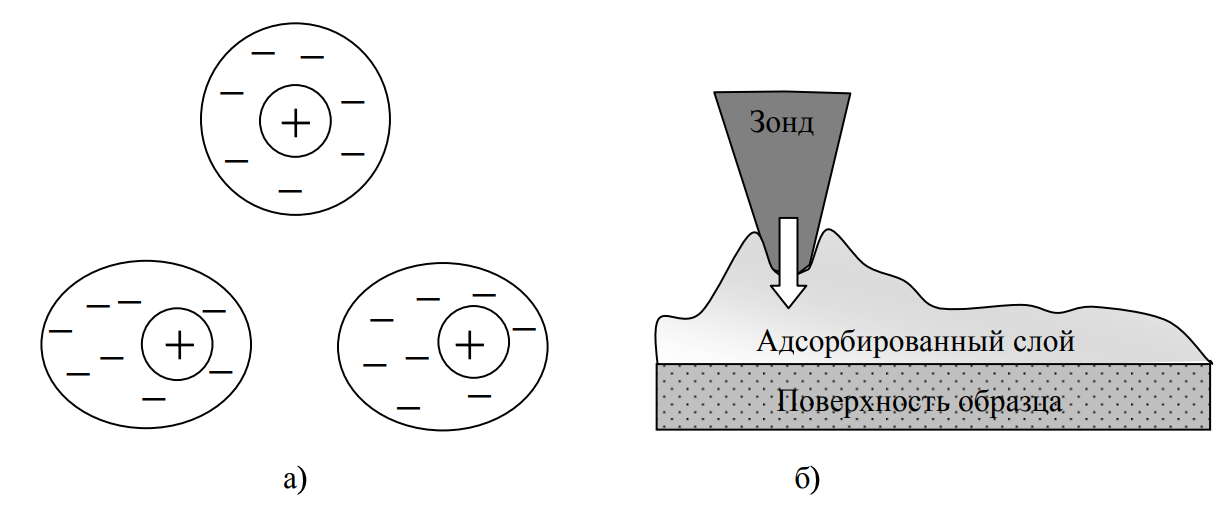
\includegraphics[width=0.5\linewidth]{pic1.png}
		\caption{{\bf {а) Притяжение двух атомов благодаря силам Ван-дер-Ваальса, б) Притяжение зонда к поверхности за счет капиллярных сил}}}
   	\label{fig:1}
\end{figure}

Если на поверхности образца имеется адсорбированный слой, то при соприкосновении зонда с его поверхностью возникает притяжение за счет капиллярных сил. Притягивающие силы могут быть обусловлены так же электростатическим взаимодействием. При дальнейшем уменьшении расстояния возникают силы отталкивания. Когда расстояние между зондом и образцом станет меньше среднего межатомного расстояния, то начнется перекрытие электронных оболочек ближайших атомов, в результате чего электроны первого атома стремятся частично занять состояния второго. В результате действия принципа запрета Паули они вынуждены занимать состояния с более высокой
энергией. Увеличение энергии системы двух взаимодействующих атомов приводит к появлению отталкивающей силы.
При еще большем сближении атомов доминирующей становится кулоновская сила отталкивания ядер

Качественно зависимость Ван-дер-Ваальсовских сил показана на рисунке 2:
\begin{figure}[H]
\centering
	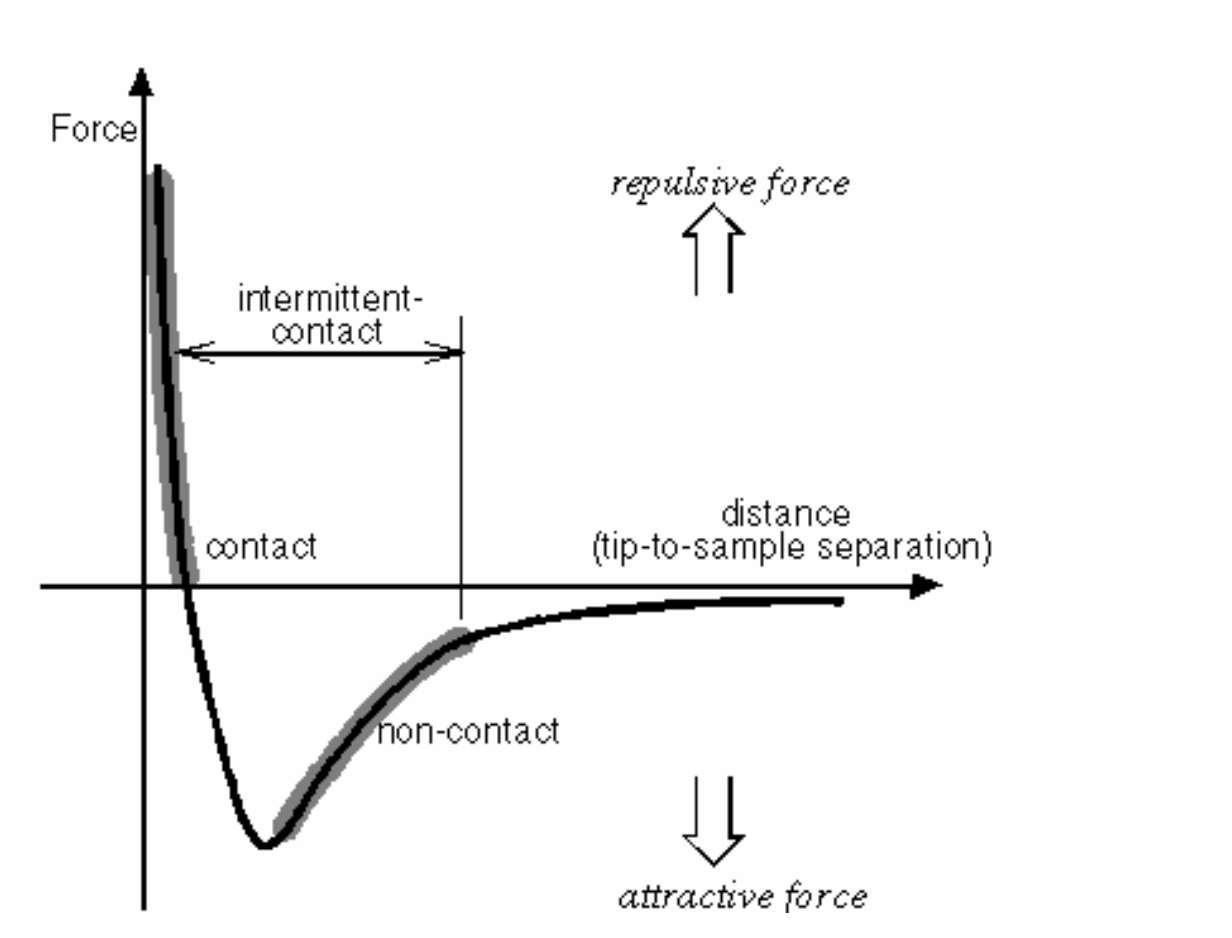
\includegraphics[width=0.6\linewidth]{pic2.png}
		\caption{{\bf {Зависимость ван-дер-ваальсовских сил от расстояния}}}
   	\label{fig:2}
\end{figure}
\subsection{Устройство АСМ}
Основными элементами микроскопа являются зонд, система регистрации отклоенеия зонда, пьезосканер, система обратной связи. На рисунке 3 представлена схема регистрации отклонения кантеливера.
\begin{figure}[H]
\centering
	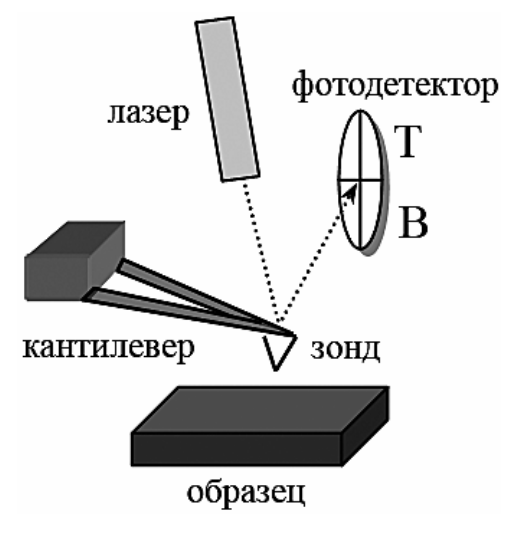
\includegraphics[width=0.3\linewidth]{pic3.png}
		\caption{{\bf {Оптическая схема регистрации отклонения кантеливера}}}
   	\label{fig:1}
\end{figure}
\subsection{Режимы работы}

\textbf{Контактный режим}
В этом режиме работы взаимодействие зонда и образца осуществляется в области действия сил отталкивания. Обычно в контактном режиме используются тонкопленочные V-образные кантилеверы из \textit{$Si_3N_4$} с пирамидальными зондами. Величина изгиба регистрируется, как правило, с помощью оптической системы (Рис. 3), состоящей из полупроводникового лазера и четырехсекционного (квадрантного) фотодиода. Оптическая система АСМ юстируется таким образом, чтобы излучение лазера фокусировалось на конце кантилевера, а отраженный луч попадал в центр фотодетектора. При изгибе кантилевера под действием контактных сил отраженный от него луч лазера смещается относительно центра фотодетектора.

\textbf{Бесконтактный режим}
В этом режиме работы зонд находится достаточно далеко от поверхности образца в области действия сил притяжения. Обычно в контактном режиме используются жесткие I-образные кремниевые кантилеверы с цилиндрическими зондами.
Силы притяжения и их градиенты слабее отталкивающих контактных сил, поэтому для их детектирования обычно используется модуляционная методика. Для этого на пьезовибратор, на котором укреплен кантилевер с зондом, прикладывается переменное напряжение (Рис. 3-7), которое вызывает изменение его геометрических размеров. Частоту переменного напряжения выбирают равной собственной частоте колебаний кантилевера. Вследствие этого кантилевер колеблется над образцом с резонансной частотой:
\begin{equation}
\omega_0 \sim \sqrt{\frac{k}{m}}
\end{equation}

где \textit{$m$} - масса кантиливера. Уравнение, описывающее движение зонда имеет вид:
\begin{equation}
\frac{d^2z}{dt^2} + \frac{w_0}{Q}*\frac{dz}{dt} + w^2_0(z-z_0) = \Delta z w^2_0 cos(\omega t)
\end{equation}
где \textit{$\omega$} - частота вынужденных колебаний пьезодрайвера, \textit{$z_0$} - расстояние от зонда до образца, \textit{$Q$} - добротность, зависящая от колебательной системы.

При \textit{$\Delta z != 0$} ищем стационарный режим колебаний с амплитудой:
\begin{equation}
\delta = \Delta z \sqrt{\frac{Q^2w^4_0}{w^2_0w^2 + Q^2(w^2_0 - w^2)^2}}
\end{equation}

Сдвиг фазы кантеливера относительно закрепленного определяется выражением:
\begin{equation}
tg(\phi) = \frac{1}{Q}\frac{w w_0}{w^2_0 - w^2}
\end{equation}

Приближение зонда к поверхности образца приводит к возникновению силы взаимодействия между ними, что эквивалентно увеличению массы зонда. Это приводит к смещению амплитудно-частотной характеристики (АЧХ) и фазо-частотной характеристики (ФЧХ) колебаний кантилевера влево по сравнению с измеренными вдали от поверхности:

 \begin{figure}[H]
\centering
	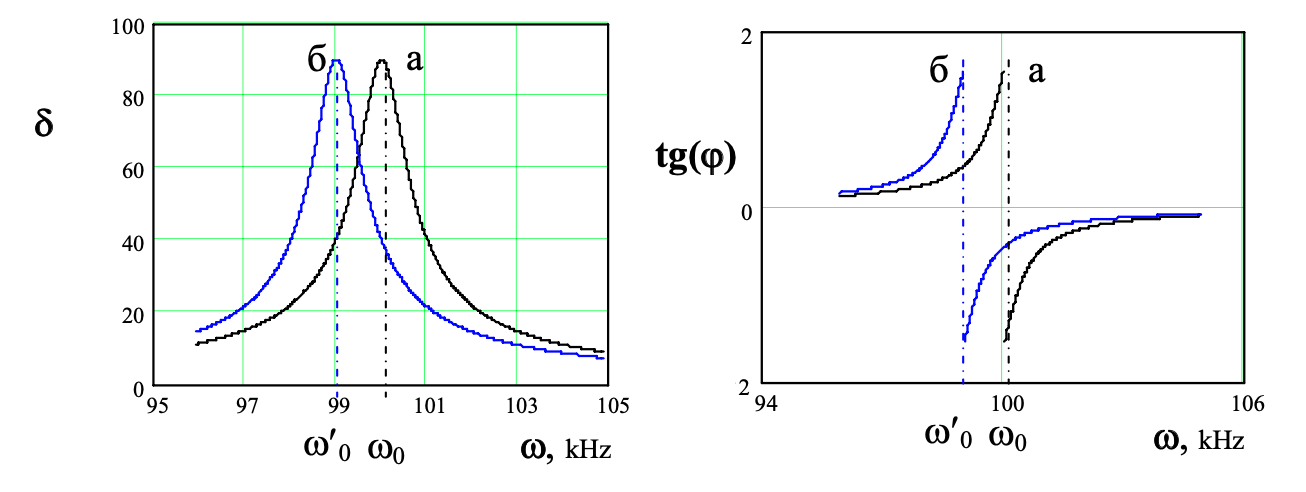
\includegraphics[width=0.9\linewidth]{pic4.png}
		\caption{{\bf {а) АЧХ, б) ФЧХ }}}
   	\label{fig:4}
\end{figure}

Резонансная частота при изменении высоты определяется выражением: 
\begin{equation}
w'_0 = w_0\sqrt{1 - \frac{1}{k}\frac{\partial F}{\partial z}}
\end{equation}

\textbf{Фазовый конраст}

Если отдельные участки поверхности имеют различные свойства, то изображение будет иметь дополнительный контраст, зависящий от природы материала на отдельных участках. Он проявляется в изменении фазы колебаний зонда, в то время как амплитуда колебаний отражает топографию поверхности. Поскольку детектирование фазы колебаний возможно одновременно с получением топографии поверхности при амплитудном детектировании положения зонда в обратной связи, то из сравнения амплитудного и фазового изображений возможно получить информацию о фазовом составе образца.


\section{Экспериментальная часть}

\subsection{Настройка резонансной частоты зонда}

Определим резонансную частоту кантеливера, график представлен на рис.5.
 \begin{figure}[H]
\centering
	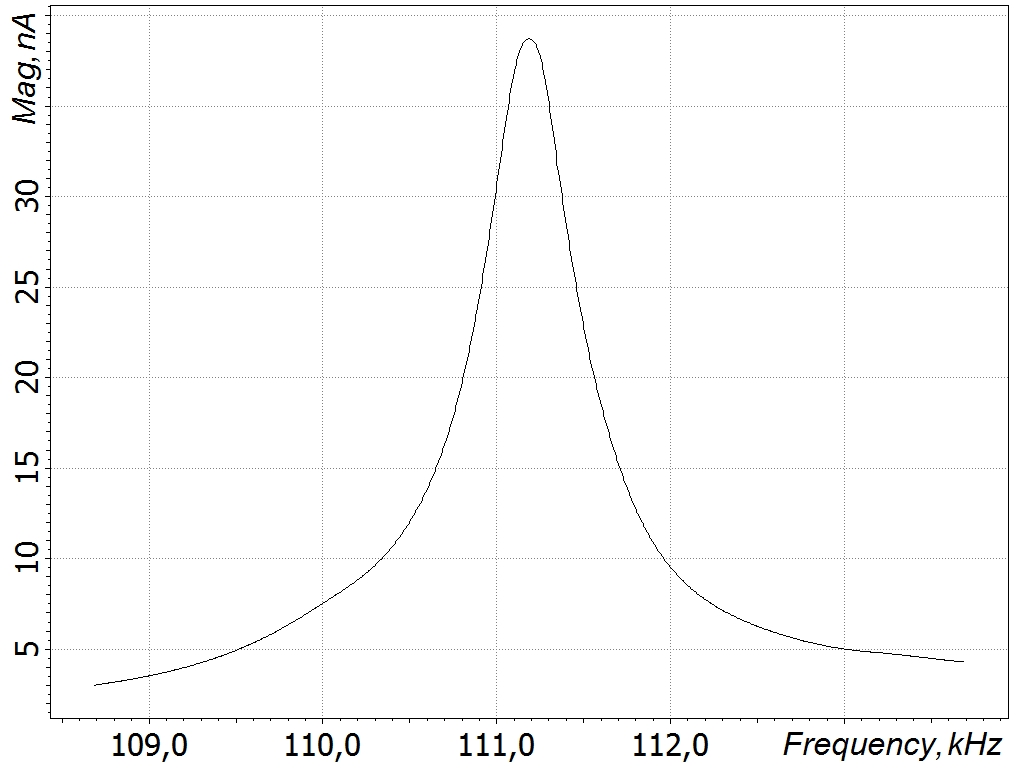
\includegraphics[width=0.8\linewidth]{curve1.jpg}
		\caption{{\bf {Резонансный пик кантеливера}}}
   	\label{fig:5}
\end{figure}
По графику определяем резонансную частоту: \textit{$w_0 = 111,18 кГц$}.

\subsection{Оценка степени остроты зонда с помощью поверхности TGT01}

Исследуем топографию образца. Получим его изображения - рис. 6, 7 и 8.
 \begin{figure}[H]
\centering
	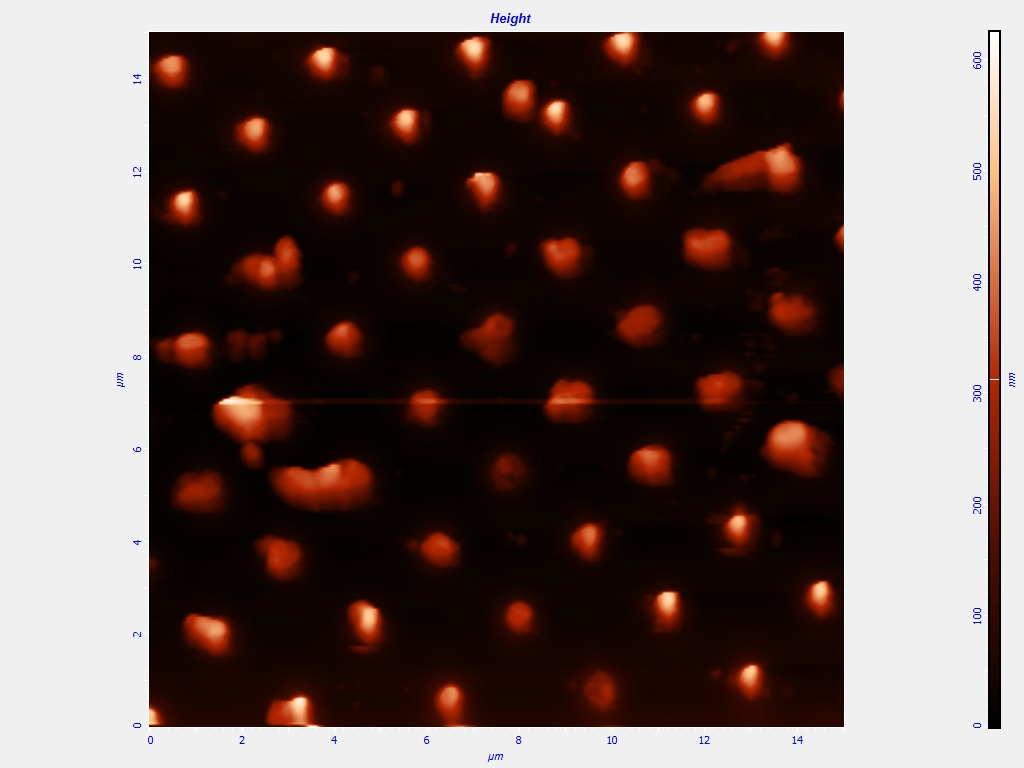
\includegraphics[width=0.8\linewidth]{ph1.jpg}
		\caption{{\bf {Изображение образца}}}
   	\label{fig:6}
\end{figure}
 \begin{figure}[H]
\centering
	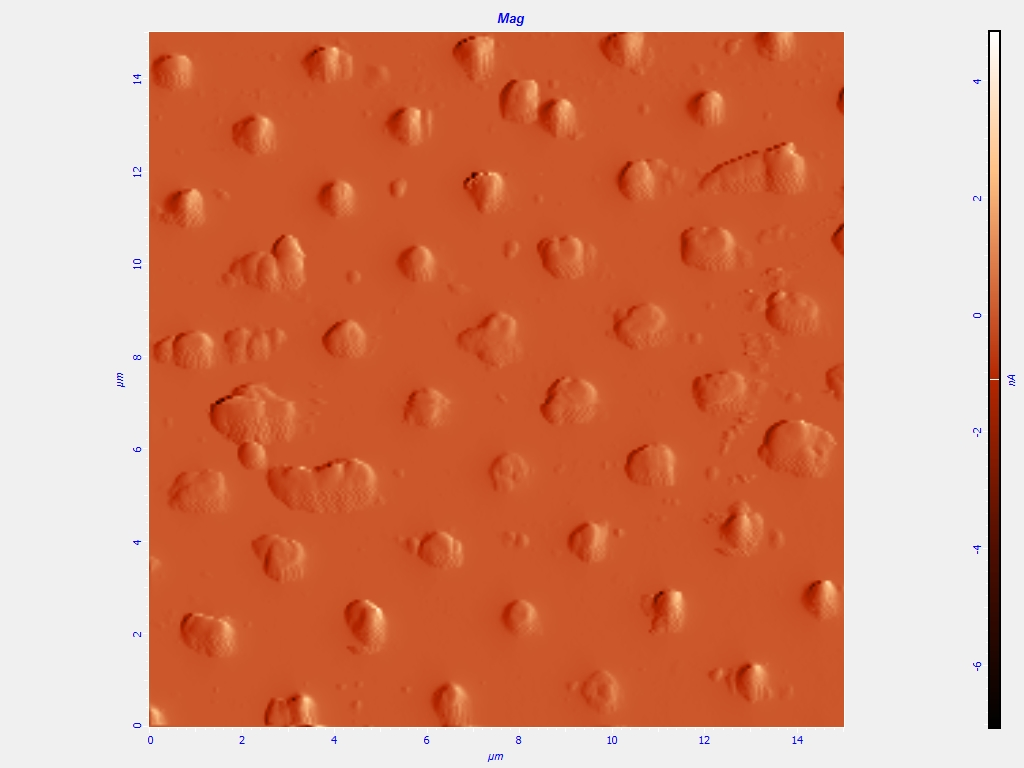
\includegraphics[width=0.8\linewidth]{ph2.jpg}
		\caption{{\bf {Распределение амплитуды}}}
   	\label{fig:7}
\end{figure}

С помощью простых инструментов обработки фотографии найдем диаметр повторяющегося объекта - величина порядка 0,9 мкм.
 \begin{figure}[H]
\centering
	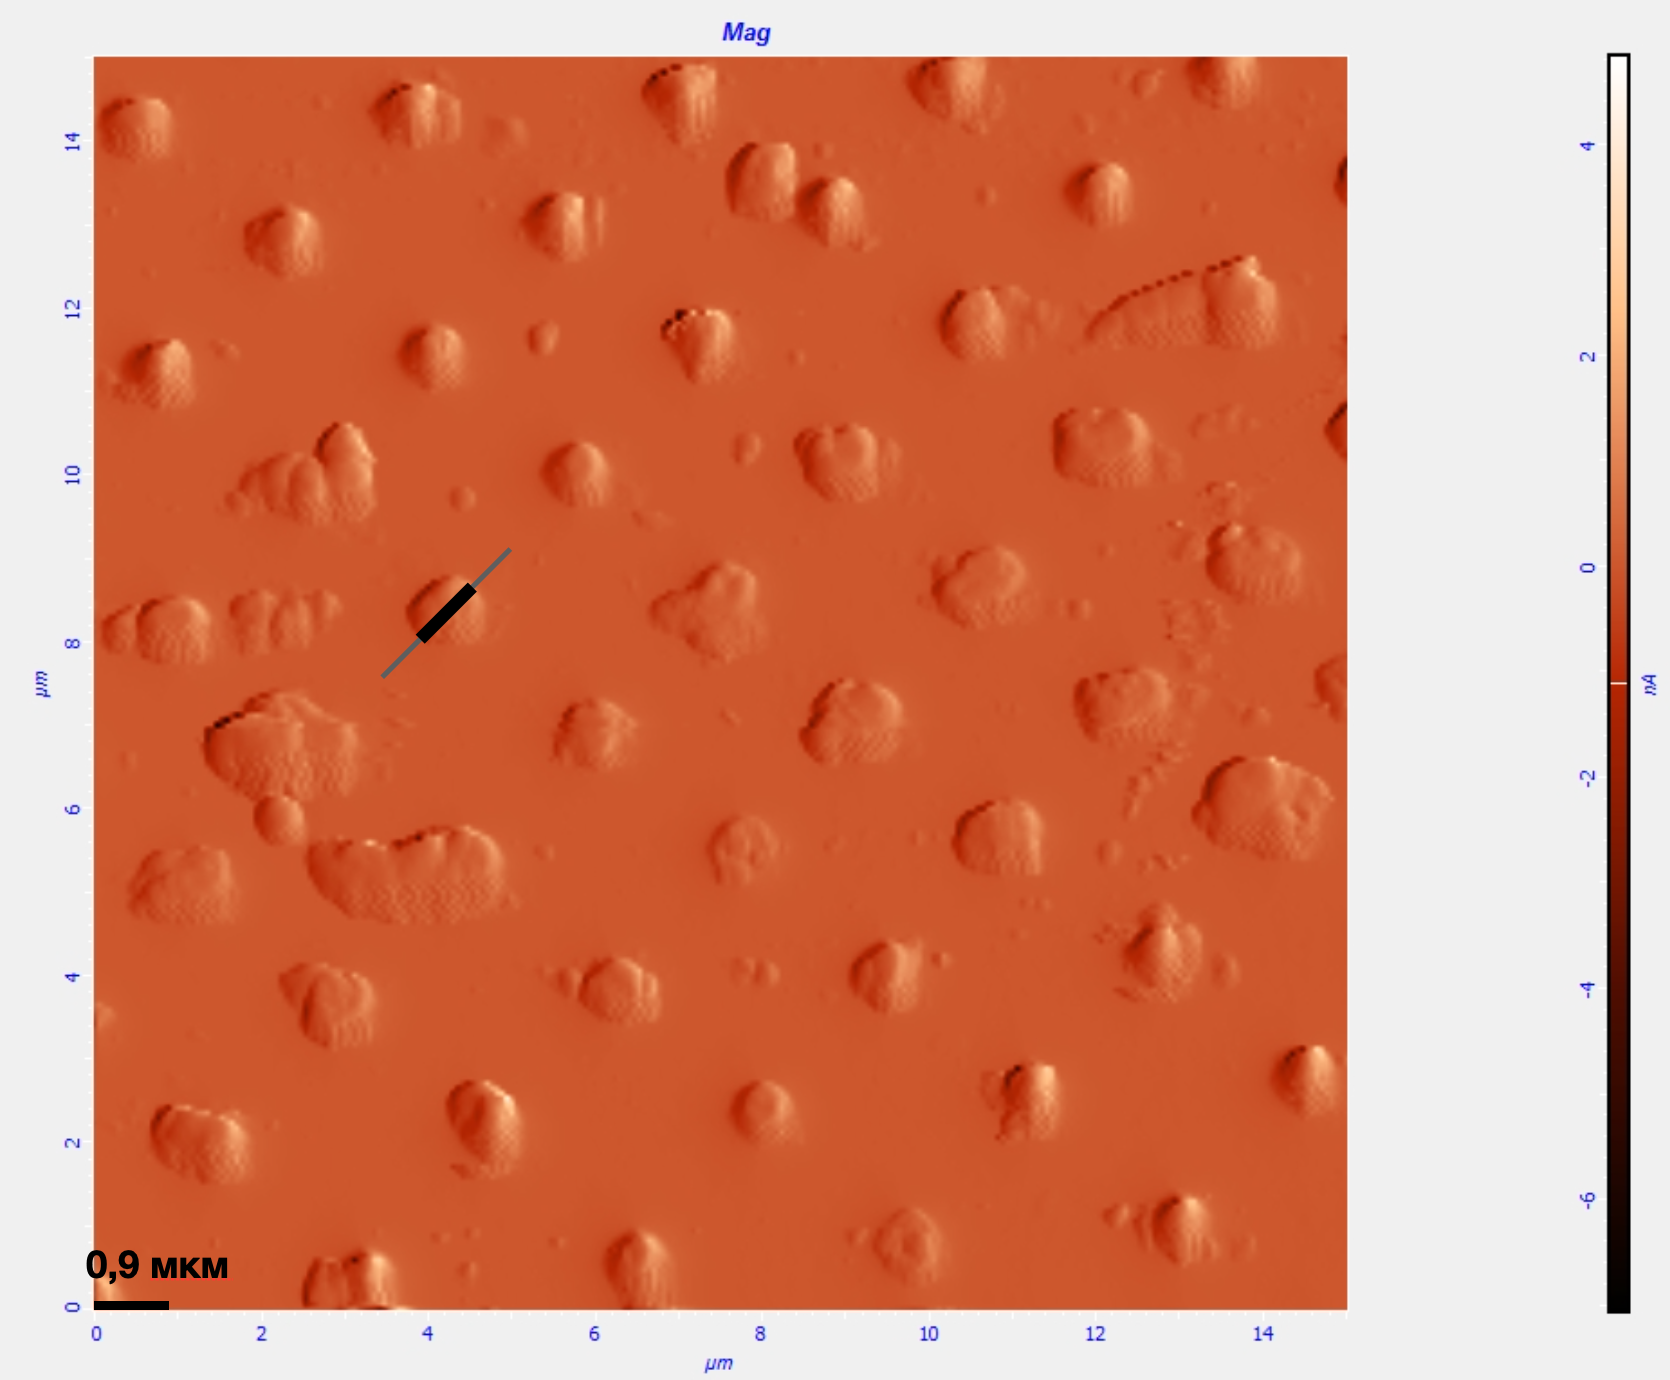
\includegraphics[width=0.6\linewidth]{anal.png}
		\caption{{\bf {Сечение иглы}}}
   	\label{fig:8}
\end{figure}

Снимем более точную величину сечения, график изображен на рис. 9:

 \begin{figure}[H]
\centering
	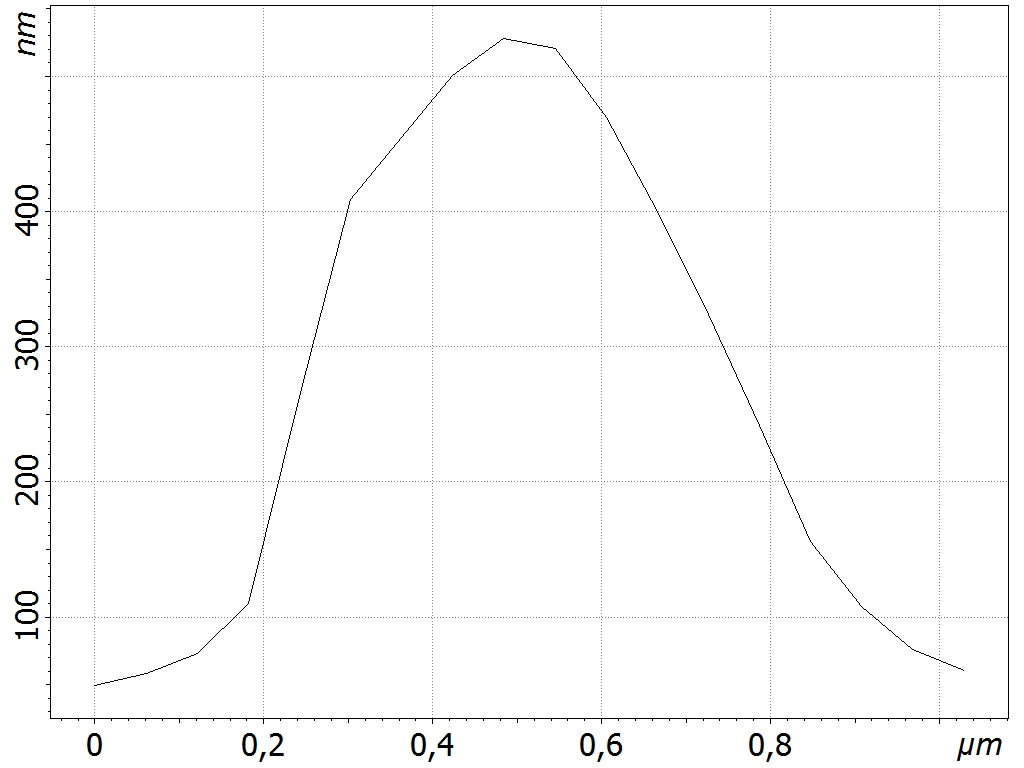
\includegraphics[width=0.6\linewidth]{curve3.jpg}
		\caption{{\bf {Сечение вдоль выступа}}}
   	\label{fig:9}
\end{figure}

\subsection{Зависимость MAG от Z}
Измерим зависимость сигнала MAG от смещения вдоль оси Z в полуконтактном режиме. График представлен на рисунке 10. На графике явно виден участок прямой пропорциональности между высотой и амплитудой кантеливера. Кроме того, на высоте порядка 0,4 - 0,5 нм заметно нелинейное поведение, обусловленное гистерезисом пъезокерамики.
 \begin{figure}[H]
\centering
	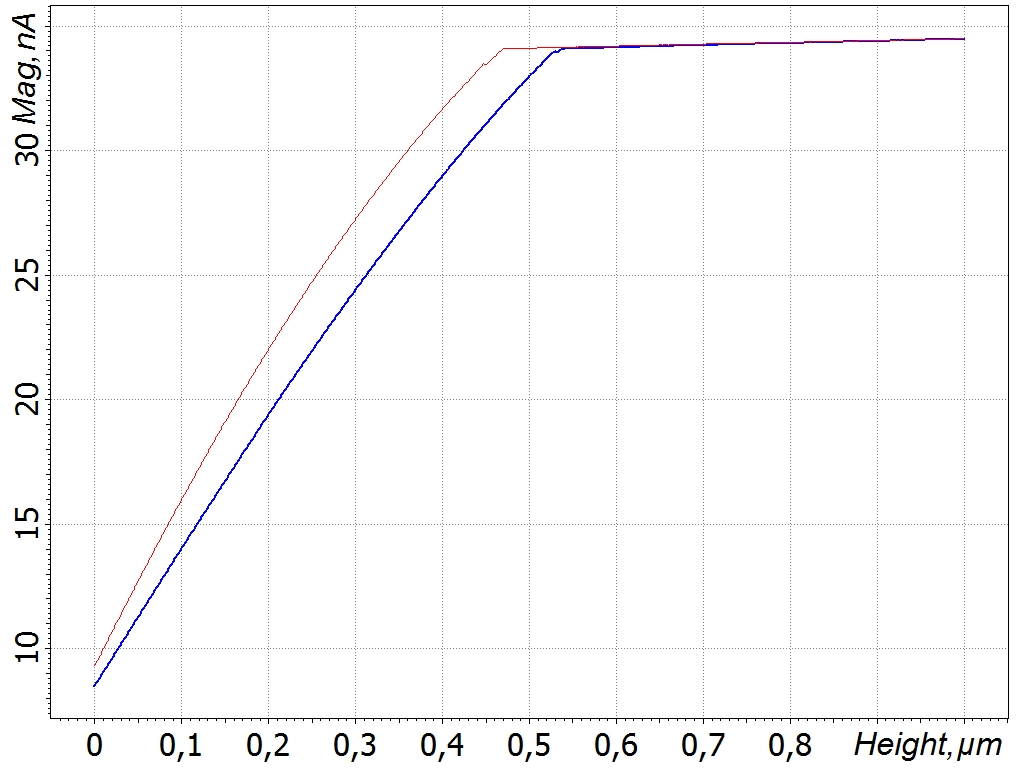
\includegraphics[width=0.6\linewidth]{curve2.jpg}
		\caption{{\bf {MAG signal depending on Z axis offset}}}
   	\label{fig:10}
\end{figure}

\section{Обработка результатов}

Для более точного определения радиуса кривизны иглы была написана программа, рассчитывающая радиус окружности по трем точкам, которые были взяты из графика на рисунке 9:
\begin{table}[h]
    \centering
    \begin{center}
    \caption{К определению радиуса кривизны иглы}
    \end{center}
    \vspace{0.1cm}
    \label{tab:my_label}
    \begin{tabular}{|p{1cm}|p{1cm}|p{1cm}|}
 \hline
 N & x, nm & y, nm\\
 \hline
1 & 420 & 500\\
 \hline
2 & 480 & 550\\
 \hline
3 & 530 & 520\\
 \hline
\end{tabular}
\end{table}

По итогу получаем \textit{$R \approx 59,2 nm$}.



\section{Вывод}
В ходе данной работы мы с коллегами на практике ознакомились с физическими принципами функционирования атомно-силового микроскопа и основными методиками измерения. 

\newpage
\section{Список Литературы}
\begin{enumerate}
\item Руководство пользователя Negra, Руководство пользователя NanoEducator. http://www.ntmdt.ru.
\item Быков В.А. Приборы и методы сканирующей зондовой микроскопии для исследования модификации поверхностей: диссертация на соискание учёной степени доктора технических наук. М., 2000. - С. 285.
\item Миронов В.Л. Основы сканирующей зондовой микроскопии. М., 2004. -144 с.
\item Бухараев А.А., Овчинников Д. В., Бухараева А.А. Диагностика поверхности с помощью сканирующей силовой микроскопии (обзор) // Заводская лаборатория. Диагностика материалов. 1997. - Т. 63. - М25. С. 10.
\item Галлямов М. О., Яминский И. В. Сканирующая зондовая микроскопия: основные принципы, анализ искажающих эффектов. http://www.nanoscopy.org.
\item Эдельман В.С. Сканирующая туннельная микроскопия (обзор) ll ПТЭ. 1989. 3Ч5. - С. 25.
\item Артюнов П.А., Толстихина А.Л., Деиидов В.Н. Система параметров для анализа шероховатости и микрорельефа поверхности материалов в сканирующей зондовой микроскопии // заводская лаборатория. Диагно-стика материалов. 1998. - Т. 65. - й 9.
\item Меры рельефные нанометрового диапазона из монокристаллического кремния. Требования к геометрическим формам, линейным размерам и выбору материала для изготовления. ГОСТ Р 8.628 - 2007.
\item Меры рельефные нанометрового диапазона с трапециедальным профилем элементов. Методика поверки. ГОСТ Р 8.629 - 2007. 13. Микроскопы сканирующие зондовые атомно-силовые измерительные. Методика поверки. ГОСТ Р 8.630 - 2007.
\end{enumerate}
\end{document}